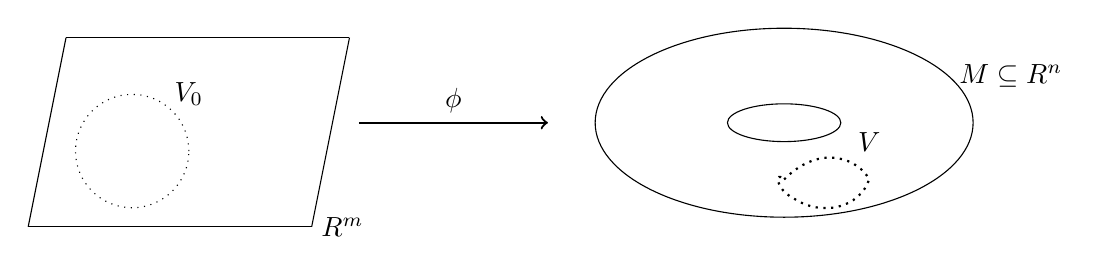
\begin{tikzpicture}[scale=1.2]

% --- Dominio en R^2 ---
\begin{scope}
  \draw[-] (0,0.4) -- (3,0.4) node[right] {$\mathbb{R}^{m}$};
  \draw[-] (0.4,2.4) -- (3.4,2.4);
  \draw[-] (3,0.4) -- (3.4,2.4);
  \draw[-] (0,0.4) -- (0.4,2.4);

  % Abierto (rectángulo)
  \draw[dotted] (1.1,1.2) circle (0.6);

  \node at (1.7,1.8) {$V_0$};
\end{scope}

% Flecha phi
\draw[->, thick] (3.5,1.5) -- (5.5,1.5) node[midway, above] {$\phi$};

% --- Toro (aproximación 2D) ---
\begin{scope}[xshift=8cm]

  % Contorno exterior (elipse grande)
  \draw (0,1.5) ellipse (2 and 1);

  % Agujero interior
  \draw (0,1.5) ellipse (0.6 and 0.2);

\draw[dotted, thick]
  (0,0.9)
  .. controls (0.4,1.3) and (0.8,1.1) ..
  (0.9,0.9)
  .. controls (0.8,0.6) and (0.4,0.5) ..
  (0.1,0.7)
  .. controls (-0.1,0.8) and (-0.1,1) ..
  cycle;

\node at (0.9,1.3) {$V$};
\node at (2.4,2) {$M\subseteq \mathbb{R}^{n}$};
\end{scope}
\end{tikzpicture}

